what is this chapter about
how is evaluation perfromed
our shader
evaluation java table generator provided by daljit.
explain how this program works:
subvariants: sample whole lambda space, just a few lambdas, pq approach.
how from those generated tables to matlab
how to read those
discussion


\section{Evaluation Data Acquisition}
\subsection{Data Acquisition}
For measurement on the true surface topography of snake sheds, samples are stuck on glass plates using double face tape, the animal was pushed up below a hollowed plate letting the skin emerging from the top of the plate. the surface of the scale under measurement should be large compared to the size of the drop to avoid wetting the plasmic membrane that would corrupt the reasing of the contact angle. 

Measurements were carried out using intermittent contact mode in a Burker Dimension 3100 atomic force microscope (AFM) under ambient conditions using a Nanoscope V controller. 

An AFM is a microscope that uses a tiny probe mounted on a cantilever to scan the surface of an object. The probe is extremely close tobut does not touchthe surface. As the probe traverses the surface, attractive and repulsive forces arising between it and the atoms on the surface induce forces on the probe that bend the cantilever. The amount of bending is measured and recorded, providing a map of the atoms on the surface. Atomic force microscopes can achieve magnification of a factor of 5 × 106, with a resolution of 2 angstroms, sufficient to resolve individual carbon atoms. Also called scanning force microscope.
is a very high-resolution type of scanning probe microscopy, with demonstrated resolution on the order of fractions of a nanometer, more than 1000 times better than the optical diffraction limit.

The tops used were etched silicon TESP tips with a nomminal frequency and force constant of 320 kHz and 42 N/m respectively. 

SHOW AFM IMAGE

\subsection{Diffraction Gratings}

The so called idealised grating is made up of a set of slits of spacing $d$. In order to cause diffraction that spacing must be wider than the wavelength of interest. Each slit in the grating acts as a quasi point source from which light propagates in all directions. The diffracted light is composed of the sum of interfering wave components emenating from each slit in the grating. 

SHOW FIGURE ABC

At any given point in space through which diffracted light may pass, the path-length to each slit in the grating will vary. Since the path-length varies, so will the phases of the waves at that point from each of the slits. This those waves will either add or subtract from one another due to the phenomenon of interference. Note that a point has maximal intensity if and only if at angleswhich would satisfy the relationship $d \frac{sin(\phi)}{\lambda} = |m|$. 

SHOW FIGURE ABC1

where m is a integer and m equal zero corresponds to specular light. 
The detailed distribution of diffraction depends on the detailed structure of the grating elements and the number of grating elements but the grating equation will always give the maximal intensity in the directions.

This derivation of the grating equation is based on an idealised grating. However, the relationship between the angles of the diffracted beams, the grating spacing and the wavelength of the light apply to any regular structure of the same spacing, because the phase relationship between light scattered from adjacent elements of the grating remains the same. The detailed distribution of the diffracted light depends on the detailed structure of the grating elements as well as on the number of elements in the grating, but it will always give maxima in the directions given by the grating equation.


MERGE ME

A diffraction grating which consists of a very large number of parallel, evenly spaced slits in an opaque sheet

A typical grating would have 10,000 slits in 1 cm and thus the slit separation is much smaller than that used in the double-slit experiment. When a beam of monochromatic light is allowed to pass through the grating placed in a spectrometer, images of the sources can be seen through the telescope at different angles.

ADD FIGURE

Since a diffraction grating is a multiple-slit plate, the maxima occur at exactly the same position as a double slit interference. However unlike a double slit, the bright fringes are sharper and brighter.

Suppose monochromatic light is directed at the grating parallel to its axis as shown. Let the distance between successive slits be d.

ADD FIGURE

The diffraction pattern on the screen is the result of the combined effects of diffraction and interference. Each slit causes diffraction, and the diffracted beams in turn interfere with one another to produce the pattern. The path difference between waves from any two adjacent slits can be found by dropping a perpendicular line between the parallel waves. By geometry, this path difference is d sin θ . If the path difference equals one wavelength or some integral multiple of a wavelength, waves from all slits will be in phase and a bright line will be observed at that point. Therefore, the condition for maxima in the interference pattern at the angle θ is 

d sin θ = n λ
where n = 0,1,2,3…..

Because d is very small for diffraction grating, a beam of monochromatic light passing through a diffraction grating is splitted into very narrow maxima(bright fringes) at large angles θ.

ADD FIGURE

The maximum number of orders that can be found by letting maximum θ = 90o and finding n using equation
n ≤ (d sin 90o)/λ

When a narrow beam of white light is directed at a diffraction grating along its axis, instead of a monochromatic bright fringe, a set of coloured spectra are observed on both sides of the central white band as shown in the Figure.

ADD FIGURE

For a diffraction grating, the condition for the nth order maximum is given by d sin θ = nλ.

Since θ increases with wavelength λ, red light which has the longest wavelength is diffracted through the largest angle. Violet light has the shortest wavelength and is diffracted the least. Thus, white light is split into its component colours from violet to red light. The spectrum is repeated in the different orders of diffraction. Only the zeroth order spectrum is pure white.

The figure below shows the difference between a monochromatic and a white light spectra.

ADD FIGURE

wo colours of different orders may overlap if their angles of diffraction θ are equal. 

MERGE ME

ADD FIGURE

The performance of a simple diffraction grating can best be shown with reference to Figure 2. Notice that the optical beam enters the periodic pattern (spatial fringe pattern) with a particular angle of incidence. The beam then separates into one or more orders according to the grating equation: EQ

Three characteristics of the simple diffraction grating stand out. As figure 2 shows, the zero order is not diffracted and therefore continues undisturbed (but has some loss of power). Also, for a given wavelength, the amount of beam turning is a function of the groove period and of the angle of incidence. Finally, no real diffracted beam exists when the wavelength is greater than twice the groove period. However, when the grove period is large compared to the wavelength many orders can exist. Indeed, Echelle gratings often operate over hundreds of orders.

Free Spectral Range:
The free spectral range of a diffraction grating is defined as the largest bandwidth in a given order which does not overlap the same bandwidth in an adjacent order. Referring to Figure 3, if ℓ1 and ℓ2 are the extremes of the spectrum band then overlapping will occur at the long wavelength end of the spectrum when ℓ2 in order m is diffracted at the same angle as in order m+1. Conversely, overlapping will occur at the short wavelength end when ℓ1 in order m coincides with ℓ2 order m-1. To avoid overlapping, the required conditions is:
ℓ2-ℓ1≦ℓ1/m or ℓ2-ℓ1≦ℓ2/(m-1)
however, since ℓ1 < ℓ2, we may say that the free spectral range is equal to the shortest wavelength in the allowed bandwidth divided by the order number.

ADD FIGURE


\subsection{Evaluation}
UNIFY ANGLE NAMES: 

In order to check the physical reliability of our method we applied it on a syntetic blazed grating, Elaphe and Xenopeltis snake sheds and evaluated its response using the grating equation. This equation models the relationship between the grating spacing and the angles of the incident and diffracted beams of light. 

When light at a wavelength $\lambda$ falls on a sample presenting a periodicity $d$ along the incident plane under an incident angle $\theta$ compared to the normal of the surface the angle $\phi$ corresponding to the direction of the emerging beam showing constructive interferences (maximum in intensity) is given by the grating equation:

\begin{equation}
  sin(\theta) = sin(\phi) + \frac{m \lambda}{d}
\end{equation}

In our evaluation we are interested in the zero order diffraction, i.e. m equals zero which corresponds to direct transmission or specular reflection in the case of a reflection grating. 
Within our evaluation we further assume that the incident light direction $w_i$ is given. In contrast the direction of the reflected wave $w_r$ is not given.
In Mathematics, a three dimensional direction vector is fully defined by two two angles, i.e. it can be represented by spherical coordinates with radius $r = 1$. By convention, we denote those two vectors by $\theta$ and $\phi$. Hence, $\theta_i$, $\phi_i$ and $\phi_r$ are given constants whereas $\theta_i$ is a free parameter for our evaluation simulation. Therefore, we are going to compare the maxima for peak viewing angle corresponding to each wavelength using data produced by our method against the maxima resulting by the grating equation.

\subsubsection{Precomputation}
SHOW IMAGE OF GRID

Before being able to compare the output produced by our method by the grating equation, we have to discretise the wavelength space $\Lambda$ and the range $\Theta$ of our free parameter $\theta_i$. We also have to initially assign  $\theta_i$, $\phi_i$ and $\phi_r$. For our experiments we choose the following initial setup: $\theta_i = 75$ $\phi_i = 0$ $\phi_r = 180$ degree.
Further we discretise the lambda space $\Lambda = \{\lambda | \lambda = \lambda_{min} + k\lambda_{step}, k \in \{0,..,C-1\}\}$ where $\lambda_{step} = \frac{\lambda_{max}-\lambda_{min}}{C-1}$ and $C$ is the discretisation level of the lambda space, in our scenario $C = 42$. We similarly discretise the angle space by predefining an minimal and maximal angle boundary and $ceil(angMax - angMin) / angInc$ is the number of angles. 
We are going implement a similar algorithm as the diffraction fragment shader algorithme on the grid $[\Lambda, \Theta]$ and will store its spectral response in a matrix $R = \{response(\lambda_i, \theta_{r}^{j}) | i index(\Lambda), j index(\Theta)\}$. We also have evaluated our other shaders, mentioned within the discussion of the derivation and implementation chapters.

\subsubsection{Data evaluation}

\begin{algorithm}
\caption{Evaluation: lambda thetar graph}
\begin{lstlisting}
% load all variables computed in java
lInc = (lMax - lMin)./(lambdaCnt-1);
lambda = lMin + lInc*(-1+[1:lambdaCnt]);
[maxC maxI] = max(response.');
viewAngForMax = angMin + angInc * (maxI-1);
plot(lambda, viewAngForMax,'-r');s

for thetaI=baseAngle-eps:0.5:baseAngle+eps,
	% grating equation
	thetaV = asin(lambda./dPeriod - sin(thetaI*pi()/180))*180/pi();
	if(thetaI==75)
		plot(lambda, thetaV,'+ b');
	else
		plot(lambda, thetaV,'. g');
	end
end

\end{lstlisting}
\end{algorithm}

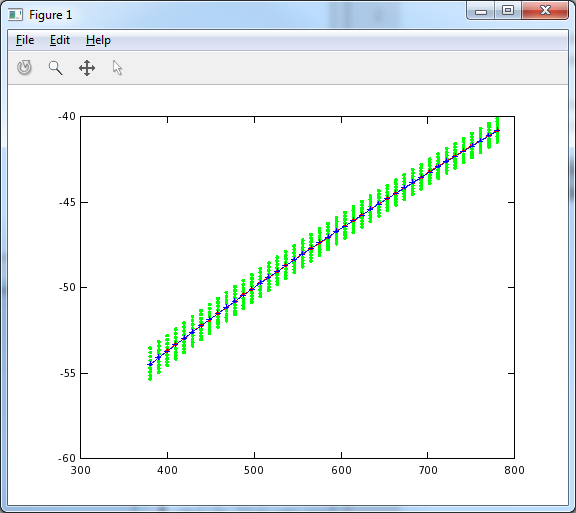
\includegraphics[scale=0.5]{images/blaze2500_75.png}
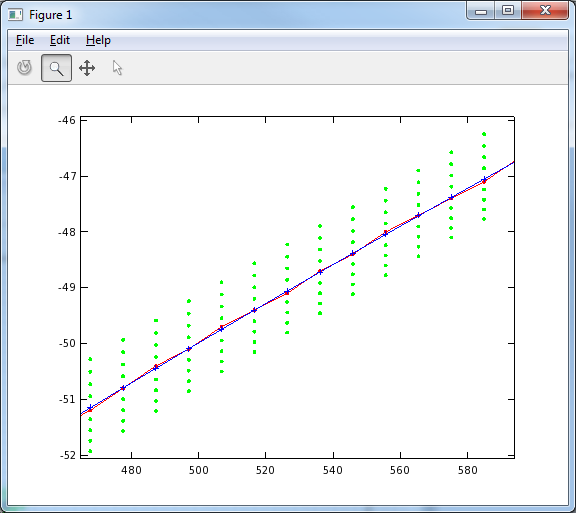
\includegraphics[scale=0.5]{images/blaze2500_75_closeup1.png}
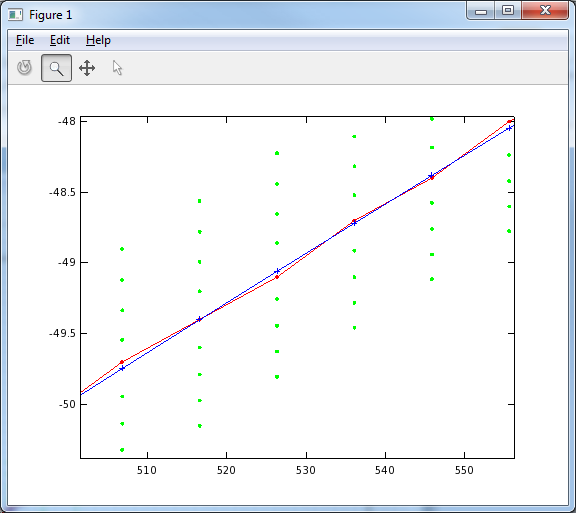
\includegraphics[scale=0.5]{images/blaze2500_75_closeup2.png}

red graph is based on data produced by our method, the blue and green graphs are plots from the grating equation for different angles. If the blue graph is close the the red one, then our method performs well. 

SHOW PLOTS AND TALK ABOUT THEM
